\documentclass{report}

\usepackage{ptext}
\usepackage{lipsum}
\input{Boostan-UserManual}
\usepackage{graphicx}
\usepackage{tabularx}

\newword{Abstraction}{Abstraction}
{انتزاع}{}

\newword{Abstract}{Abstract}
{انتزاعی}{}

\newword{AbsoluteMinimum}{Absolute Minimum}
{کمینه مطلق}{}


\newword{AcceptableCell}{Acceptable Cell}
{سلول پذیرفتنی}{سلول‌های پذیرفتنی}

\newword{AccessBurst}{Access Burst}
{توده دسترسی}{توده‌های دسترسی}


%%% S
\newword{Sample}{Sample}
{نمونه}{نمونه‌ها}

\newword{SamplePath}{Sample Path}
{نمونه مسیر}{}

\newword{SampleSpace}{Sample Space}
{فضای نمونه}{فضای نمونه‌ها}
\newacronym{ACK}{ACK}{Acknowledgement}

\newacronym{ACI}{ACI}{Application Control Interface}

\newacronym{ACIR}{ACIR}{Adjacent Channel Interference Ratio}

\newacronym{ACLC}{ACLC}{Adaptive Configuration of Logical Channels}

\newacronym{ACLP}{ACLP}{Adjacent Channel Leakage Power}

\title{پروژه باریم
}
\type{
 درس آشنایی با شبکه های تلفن همراه }
\author{غزل عربعلی - 97521396، بهاره کاوسی نژاد - 99431217}
\logofile{Pic/IUST}


\begin{document}
\pagenumbering{gobble}
\maketitle
\pagenumbering{arabic}
\chapter{شرح پروژه}


گسترش روزافزون شبکه های تلفن همراه به ویژه شبکه های نسل چهار و پنج، موجب شده است که این شبکه ها به عنوان بزرگترین شبکه دسترسی
\footnote{\lr{Access Network}}
 ، برای دستیابی به خدمات اینترنت بشمار آید. پرواضح است که در این بین، مساله امنیت
 \footnote{\lr{Security}}
  برنامه های کاربردی
  \footnote{\lr{Application}}
  و ساخت یک برنامه کاربردی با یک ارتباط امن، یکی از مهم ترین مسایل این حوزه خواهد بود. گرچه باید به این نکته توجه داشت که امنیت در یک ارتباط از طریق شبکه های تلفن همراه را، نباید تنها به مساله امنیت در دو سوی مشتری
   \footnote{\lr{Client}}
   و خدمت گزار
   \footnote{\lr{Server}}
   تقلیل داد؛ بلکه در جای جای این ارتباط، ما می توانیم با حملات متعددی مواجه شویم، که می تواند محرمانگی
   \footnote{\lr{Confidentiality}}
   ، یکپارچگی
   \footnote{\lr{Integrity}}
    و حریم خصوصی
    \footnote{\lr{Privacy}}
     ما را هدف قرار دهد. شکل 
     \ref{fig:Client_Server}
      نمایی از ارتباط یک مشتری با خدمت گزار را در بستر های مختلف از طریق شبکه های تلفن همراه به زیبایی نشان می دهد.
  
   \begin{figure}[ht]
   	\centering
   	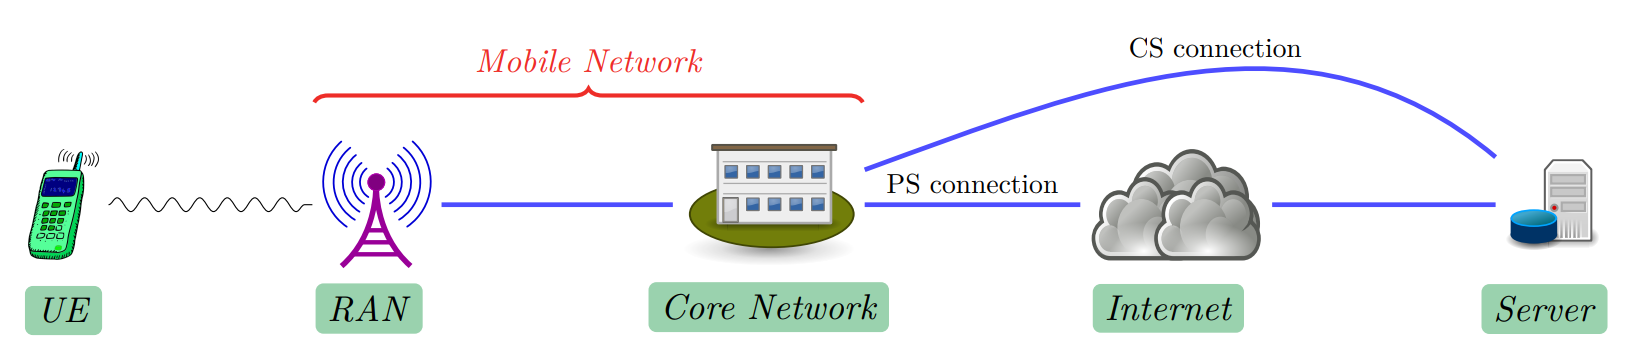
\includegraphics[width=\textwidth]{Pic/Client_Server}
   	\caption{ارتباط بین مشتری با خدمت گزار از طریق شبکه های تلفن همراه بر روی بسترهای مختلف}
   	\label{fig:Client_Server}
   \end{figure}
   
   در مساله پیش رو، فرض می کنیم که یک برنامه کاربردی داریم، که توسط برنامه 
   \lr{UE}
    می شود.
     \lr{UE}
      از دیدگاه ما هر ابزاری است که توسط آن بتوان به شبکه های تلفن همراه متصل شد.
       \lr{UE}
        می تواند گوشی تلفن همراه، تبلت و یا حتی هر شی در
         \lr{IoT}
         \footnote{\lr{Internet of Things}}
          باشد. گرچه در این پروژه، ما تنها بر روی گوشی های تلفن همراه و تبلت ها تمرکز خواهیم کرد.
          
   برنامه کاربردی
   \lr{UE}
    قرار است تا از طریق بسترهای موجود در شبکه های تلفن همراه به یک خدمت گزار مشخص متصل شوند و با آن تبادل اطلاعات داشته باشند. در این جا ما دو راه کار برای اتصال به خدمت گزار داریم. در راه کار نخست و بدیهی ترین شیوه، ما از طریق بستر اینترنت با خدمت گزار به تبادل داده مبادرت می ورزیم. ما اصطلاحا به این شیوه اتصال از طریق 
    \lr{PS}
    \footnote{\lr{Packet-switched}}
     می گوییم. بالاخره باید پذیرفت که دنیای اینترنت، مخاطرات پیدا و پنهان فراوانی دارد. اتصال از طریق خدمات
     \footnote{\lr{Service}} 
     \lr{CS}
     \footnote{\lr{Circuit-switched}}     
     نظیر تماس
     \footnote{\lr{Call}}
      و 
      \lr{SMS}
      \footnote{\lr{Short Message Service}}
     ، می تواند راه فراری از مخاطرات دنیای اینترنت باشد. در این پروژه، ما فرض می کنیم که اتصال مشتری به خدمت گزار را از طریق
      \lr{SMS}
      ، برقرار خواهد شد.
      
     \begin{figure}[ht]
     	\centering
     	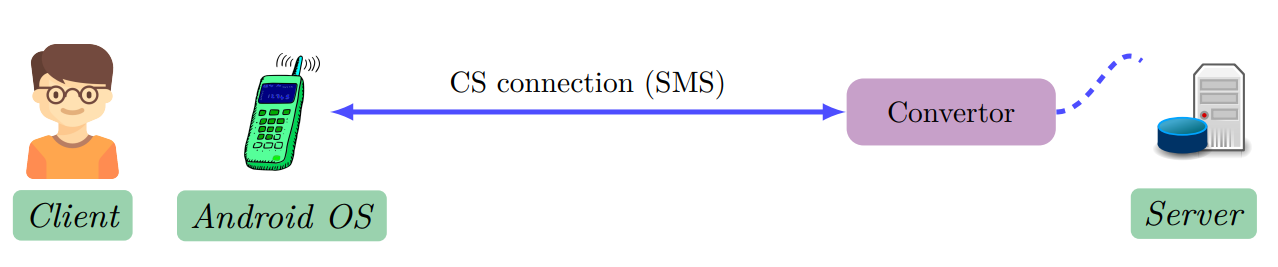
\includegraphics[width=\textwidth]{Pic/High_level_architecture}
     	\caption{معماری سطح بالای سامانه}
     	\label{fig:High_level_architecture}
     \end{figure} 

در این جا برای سادگی فرض کنید که دو گوشی داریم. گوشی سمت مشتری و گوشی که ما به عنوان خدمت گزار از آن استفاده می کنیم. در سمت خدمت گزار (که در حقیقت یک گوشی معمولی است)، یک برنامه
 \lr{Android}
 ای با کارکرد
  \lr{Backend} 
  نصب می شود.
مشتری از طریق
 \lr{SMS}
  فرمان ها را به سمت مقابل (خدمت گزار) ارسال می کند. مشتری می بایست به صورت مداوم اطلاعات مربوط به توان دریافتی و تکنولوژی سلول خدمتگزار
  \footnote{\lr{Serving Cell}}
  و مکان دریافت این اطلاعات را در صورتی که توان از یک سطح آستانه معین پایین بیاید در قالب یک پیام برای خدمت گزار ارسال کند. در این سامانه می بایست به نکات زیر دقت کنید:
  \begin{itemize}
  	\item
  	برنامه سمت خدمت گزار می بایست به صورت یک سرویس در 
  	\lr{Android} 
  	باشد، البته برای مدیریت و پیکربندی آن می توان یک برنامه
  	\lr{UI}
  	 دار نیز داشته باشیم.
  	\item
  	فرض کنید که همگان پروتکل ارتباطی شما را که مبتنی بر
  	 \lr{SMS}
  	  است می دانند. اگر اجازه دهیم
  	   \lr{SMS}
  	    از هر شماره ای به سمت خدمت گزار ارسال شود، رویه ای در نظر بگیرید که جلوی دسترسی های غیرمجاز را بگیرد. شاید یک رویه ساده، ارسال یک رمز عبور
  	    \footnote{\lr{Password}}
  	     در ابتدای
  	    \lr{SMS}
  	     است. تلاش کنید تا رویه های بهتری برای حل این چالش در نظر بگیرید.
  	\item
  	در هنگامی که مشتری درخواست خود را برای خدمت گزار ارسال می کند، خدمت گزار درخواست را می بایست اجرا کند و پاسخ را در یک
  	\lr{SMS}
  	 جداگانه برای مشتری ارسال کند. دقت کنید اگر بتوانید باید تشخیص بدهید که 
  	 \lr{Delivery}
  	 بر می گردد یا خیر. اگر برنگشت باید پیام را دوباره ارسال کنیم.
  	\item
  	در پیام ارسالی از سوی مشتری، می بایست مکان اندازه گیری، مقداری اندازه گیری و اطلاعات سلولی که به آن متصل است را ارسال کند.
  	\item 
  	پروتکل ارتباطی را باید به صورت کامل مستند بکنید، و باید مبتنی بر پروتکل 
  	\lr{SMPP}
  	\footnote{\lr{Short Message Peer-to-Peer}}
  	 باشد.
  \end{itemize}


\chapter {مراجع}
\begin{itemize}
	\item 1
\end{itemize}
\end{document}
